\documentclass[11pt, oneside]{article}   	% use "amsart" instead of "article" for AMSLaTeX format
\usepackage{geometry}                		% See geometry.pdf to learn the layout options. There are lots.
\geometry{letterpaper}                   		% ... or a4paper or a5paper or ... 
%\geometry{landscape}                		% Activate for rotated page geometry
%\usepackage[parfill]{parskip}    		% Activate to begin paragraphs with an empty line rather than an indent
\usepackage{graphicx}				% Use pdf, png, jpg, or eps§ with pdflatex; use eps in DVI mode
								% TeX will automatically convert eps --> pdf in pdflatex		
\usepackage{amssymb}

%SetFonts

%SetFonts


\title{SitePassword Modulo Bias}
\author{Alan H. Karp}
%\date{}							% Activate to display a given date or no date

\begin{document}
\maketitle
\abstract

SitePassword hashes  a super password, a per site nickname, and a per site userid to produce a site password.  The bytes produced by the hash need to be converted to a string of characters selected from the alphabet supported by the web site associated with that user account.  In some situations, {\em modulo bias} reduces the entropy of the site password.  This note shows that the effect is small enough to ignore for the range of values SitePassword supports.

\section{Introduction}

SitePassword uses each byte of the hash produced by PBKDF2\footnote{Password Based Key Derivation Function} to compute the $i$-th character of the site password using $c_i = A[b_i\%|A|]$, where $A$ is an array of characters representing the alphabet, $b_i$ is the byte value, $\%$ represents modulus, and $|A|$ is the size of the alphabet.  If the size of the alphabet evenly divides $2^8 = 256$, every character in the alphabet has the same probability of being selected.  If it doesn't, then some characters have a higher probability than others.  This {\em modulo bias} reduces the entropy of the resulting string.  This document shows that modulo bias does not have a substantial effect on the guessability of the site password it generates.

\section{Recommended Approaches}

The recommended approach to eliminating modulo bias is {\em rejection sampling}.  Simply ignore any byte value index outside the range of the alphabet.  In other words, don't use any $b_i > |A|$.  Theoretically, this approach could require an unbounded number of bytes, but the number of bytes needed is quite modest in practice.  The recommended approach to mitigating modulo bias is to use a larger range of random numbers, say two bytes instead of one.  There is still bias, but the effect on guessability is orders of magnitude smaller.

Unfortunately, while these approaches make it harder to guess the site password, they both make it easier to guess the super password.  Say that an adversary has learned a user's id and site password for a single site, perhaps from a breach, and can guess the site nickname.  The adversary can then mount an offline guessing attack to try to learn the user's super password.  As described in the Collisions document, that adversary has to try many guesses online if the entropy of the user's super password is greater than that of the site password.  Unfortunately, the more bytes used to calculate the site password, the fewer guesses the adversary has to try online.

\section{Quantifying Modulo Bias}

There will be no need to use extra bytes to construct the site password if modulo bias doesn't weaken the site password very much.  One way to quantify that weakening is by looking at the entropy of the site password both with and without modulo bias.  Without bias, the entropy of an $L$-character site password is

\begin{equation}
E_0 = L \log_2 |A|
\end{equation}

The easiest way to understand modulo bias is to repeat the alphabet until the result is has more elements than the largest possible random value $R$ and truncate to size $R$.  We see that some numbers may appear one more time than others.
\begin{eqnarray}
n_1 = \lfloor R/|A| \rfloor \\
n_2 = \lceil R/|A| \rceil,
\end{eqnarray}
so that $n_1 = n_2$ if $|A|$ divides $R$ or $n_2 = n_1 + 1$ otherwise.  The probabilities that one of those characters is chosen is, 
\begin{eqnarray}
p_1 = n_1/R \\
p_2 = n_2/R.
\end{eqnarray}

The entropy of selecting a single character from each subset is then
\begin{eqnarray}
E_1 = -(|A| - R\%|A]) p_1 \log_2 p_1 \\ 
E_2 = - (R\%|A|) p_2 \log_2 p_2.
\end{eqnarray}

Here $R\%|A|$ is the number of characters that appear an extra time.  Note that if $|A|$ divides $R$, $E_2 = 0$ and $E_1 = E_0$.  The entropy of an $L$-character site password with modulo bias is $E_b = L(E_1 + E_2)$.  

\begin{figure}
    \centering
    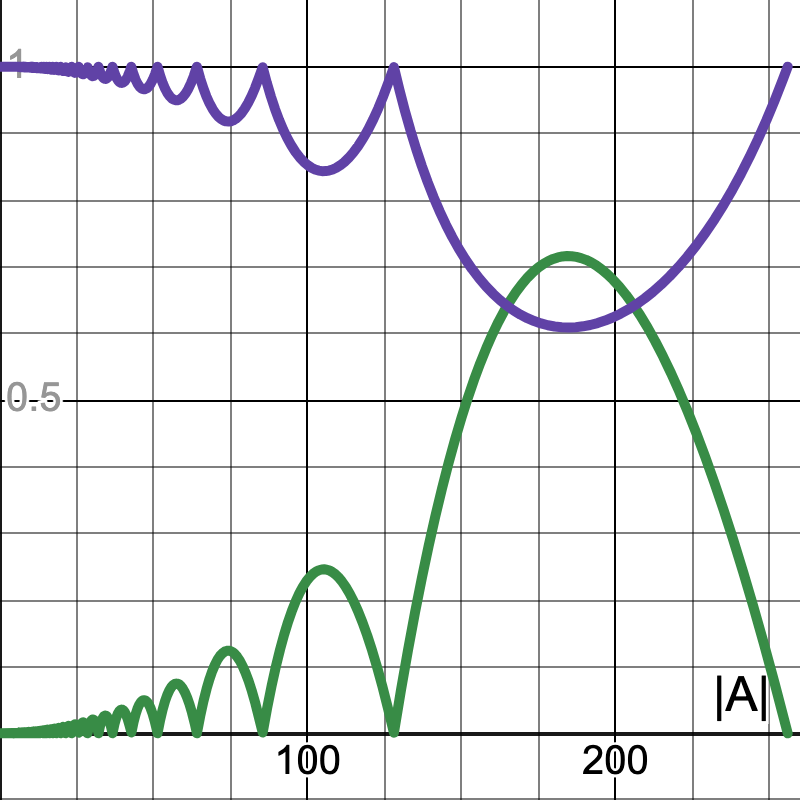
\includegraphics[width=0.5\textwidth]{moduloBias.png} 
    \caption{Modulo bias for SitePassword for an $L$-character site password.  The green line is the entropy loss; the purple line the reduction in the number of guesses.  Only values of $10 \leq |A| \leq 96$ are relevant to SitePassword.}
    \label{fig}
\end{figure}

We can now plug in some numbers.  SitePassword uses $R = 256$ and allows alphabets in the range $10 \leq |A| \leq 96$ with a default of $|A| = 62$ and $L = 12$.  With the default values $E_0 - E_b = .05$ or 96\% of the $2^{71}$ guesses needed if there was no modulo bias.  The worst case in the allowed range is at $|A| = 96$ where $E_0 - E_b = 0.28$, which translates into 82\% as many guesses.  The greater loss in guesses is offset by the larger alphabet size leaving the entropy with modulo bias greater than 78 bits.  Figure~\ref{fig} shows the entropy loss, $E_0 - E_b$, in green and the ratio of the number of guesses needed, $2^{-(E_0-E_b)}$, in purple for $R = 256$ and $L = 12$.

\section{Conclusions}

There are cases where a small modulo bias can be a serious problem, such as in choosing a nonce for a stream cypher.  That is not the case for SitePassword.  Even the most extreme bias reduces the entropy of the site password by less than a bit.

\end{document}  